Library generation is the process of creating of a large set of primitives $P$, each of which define a trajectory $\Phi(\theta^+) \to \Phi(\theta^-)$, where $\Phi(\theta^+), \Phi(\theta^-) \in \tilde{Q}$, the set of all impact configurations. Note that we define $\tilde{Q}$ with $q\equiv Rq$. That is, a final configuration is considered equivalent to the initial configuration to which it maps through an impact event. The library is intended to be structured such that efficient on-line use is enabled. Minimising off-line computation time is a secondary concern.

\subsection{Acceptable coverage}
As motivated in the previous section, a useful library of motion primitives for walking over uneven terrain requires coverage over the start and final configurations of the robot along with a range of kinetic energy additions and subtractions. Depending on the unevenness of the terrain, a diverse range of paths of the end of the swing leg may also be required. All generated constraints should be admissible and usable to avoid wasted memory and computation time.

While it is clear that some density of coverage is required, it is not immediately obvious what constitutes sufficiency. It is advantageous to avoid over-populating the library in order to speed up its generation and real-time use and reduce the memory requirements. However, advantages in computation time are meaningless if the library is insufficient for its purpose. As a result, methods for defining acceptable coverage of the dimensions of this optimisation are required.

\subsubsection{Start and end configurations}
It is essential that the library is designed such that final configurations of virtual constraints match initial configurations of other constraints through the impact map. A primitive is not useful if there are no primitives which can succeed it. Other than a detailed study of the terrain on which the robot is intended to be used, there is no good means for deciding on sets of configurations which should be reachable through a single constraint from a given configuration, therefore it seems necessary to generate a set of virtual constraints linking each pair in $\tilde{Q}\times\tilde{Q}$. This provides further motivation to avoid specifying more impact configurations than necessary, since the number of virtual constraints in the library $\lvert P \rvert \propto \lvert\tilde{Q}\rvert^2$.

The most important consideration for impact configuration coverage is to ensure that there is a relatively fine grid of vertical displacements $p_v(\theta^-)$ for a given horizontal displacement to allow for the traversal of the robot over unpredictable terrain. The resolution and bounds of this grid should chosen be such that the intended terrain is properly discretised; large gaps between the upper/lower bounds and the maximum displacement of the expected terrain should be avoided. Certainly, the upper and lower bounds should not exceed the capability of the robot. Furthermore, the resolution should be comparable in size to the combined error in the robot's perception of the terrain and the closeness to which the controller can regulate a trajectory. As is evident from these requirements, the best choice of grid for height values depends on the terrain and robot for which the library is being designed. We denote the number of unique step heights $n_y$.

It is much less important to have a dense grid of horizontal displacements. Indeed, dynamic walking over uneven terrain in most instances achievable with a fixed step length. This fact forms the basis of much of the previous work using feedback-stabilised periodic gaits to enable locomotion over relatively uneven terrain \cite{bigdog?}. Having a set of step lengths is advantageous in that it enables for intelligent foot placement. Denote the number of unique step lengths $n_x$.

Other than in the case of the compass-gait robot, the step length and height are not sufficient to specify the final configuration of the robot. It is therefore necessary to perform inverse kinematics to generate joint angles. In the general case, there are infinitely many combinations of joint angles which can produce the final configuration for a particular step length and height. There is no general method for producing the best configuration; it depends on the robot's mechanical design and the desired gait. While not strictly necessary for terrain scalability, the energy efficiency of planned trajectories can be improved by having multiple configurations of joints per step length and height from which to choose. Let us denote the number of these configurations $n_q$.

The cardinality of the set of all impact configurations is trivially evaluable:
\begin{equation} \label{eqn:numimpactconfs}
\lvert\tilde{Q}\rvert = n_xn_yn_q
\end{equation}
We note that while $n_q$ must be fairly large to enable walking over uneven terrain, $n_x$ and $n_q$ are useful only to provide additional control and should be kept small.

\subsubsection{Inter-step kinetic energy changes}
The only method of velocity control available to the motion planner is to chose constraints which add, maintain or reduce the kinetic energy of the walker. It is therefore important to produce, for each pair of step length and height, a range of kinetic energy mutations. For simplicity, we produce a set of kinetic energy additions and subtractions $\tilde{K}$, where $\lvert\tilde{K}\rvert = n_k$. For each set of initial and final configurations $q^+,q^- \in \tilde{Q}$, we produce the $n_k$ unique trajectories $q^+ \to q^-$ with $\Delta$KE $\in \tilde{K}$. We therefore may formulate an expression for the total number of primitives in the library:
\begin{equation}
	\lvert P \rvert = n_k\left( n_xn_yn_q\right)^2
\end{equation}

For a given robot, it may be possible to define a particular range of $\Delta$KE values on the basis of the initial and final configuration. For instance, since a step-up trajectory converts kinetic into potential energy, constraints which add the maximum kinetic energy may not ever be chosen by the motion planning algorithm. Such reasoning is difficult to properly justify in general and as such has not been pursued in this thesis work. Even if such reasoning is used, it is still likely best to produce $n_k$ paths.

We need not be as strict on keeping $n_k$ small, since $\lvert P \rvert \propto n_k$ rather than $n_k^2$, however since velocity control is able to be executed over multiple footsteps, the precision and variety of $\Delta$KE over a single footstep is not critical. Therefore in the interest of keeping the library manageable, $n_k$ should be kept to a moderate size.

Note that while the initial and final configurations are important data for a virtual constraint, the target $\Delta$KE should not be stored. As discussed previously, the change in kinetic energy is dependent on the initial velocity of the constraint. Furthermore, its calculation requires very little computation due to the affine form of the partial solution.

\subsubsection{Ground configurations} \label{sec:ground}
It is important to consider the likely shape of the ground for constraints with particular step lengths and heights. For the off-line generation of virtual constraints, it is best to be somewhat conservative in specifying where the ground level changes. Consider Figure \ref{fig:stepup}; the terrain steps up at a horizontal displacement significantly smaller than $p_h(\theta^-)$. It is reasonable to expect that this is representative of the typical use case of a step-up virtual constraint. It is not necessary to optimise numerous primitives with all else fixed but with varied ground configurations; if the terrain profile for the purposes of each single VC optimisation is conservatively defined, the ground configuration is indirectly sampled by producing constraints with varying initial and final configurations.

\begin{figure}
	\centering
	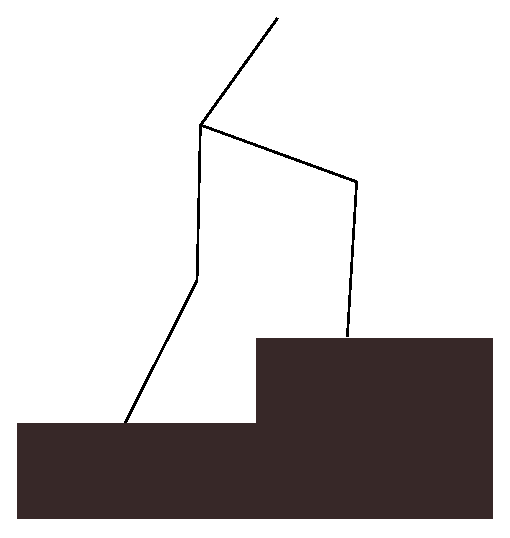
\includegraphics[width=0.5\linewidth]{4VirtConstLib/stepup.eps}
	\caption{Example step-up showing possible terrain profile}
	\label{fig:stepup}
\end{figure}

\subsection{Ordering sets of constraints} \label{sec:orderings}
As discussed in Section \ref{sec:primplanning}, planning with primitives is made much more efficient if there is a means of ordering the primitives, since this facilitates a binary search, reducing the worst-case search time from $O(n)$ to $O(\log n)$. As discussed in \cite{manchester13planning}, the partial solution for velocity avails a method of ordering sets of constraints on the basis of a desired critical velocity $\dot{\theta}_a$. Recall that the velocity at the critical point for the constraint $\alpha$ is given by:
\[
	\dot{\theta}_c^2 = \Gamma(\theta_\alpha^c)\dot{\theta}_0^2 + \Psi(\theta_\alpha^c)
\]
If we say that we wish for the constraint to pass through the critical point with minimum velocity $\dot{\theta}_a$, then
\begin{align*}
	\Gamma(\theta_\alpha^c)\dot{\theta}_0^2 + \Psi(\theta_\alpha^c) &\geq \dot{\theta}_a^2 \\
	\dot{\theta}_0^2 \geq \frac{\dot{\theta}_a^2 - \Psi(\theta_\alpha^c)}{\Gamma(\theta_\alpha^c)}
\end{align*}
We construct a precedence $\alpha \prec_{\dot{\theta}_a} \beta$ on the basis of the minimum required initial velocity $\dot{\theta}_0^2$ to achieve $\dot{\theta}_c\geq\dot{\theta}_a$:

\begin{figure}[h]
\centering
$\alpha \prec_{\dot{\theta}_a} \beta$ if $q_\alpha^-=q_\beta^-$, $q_\alpha^+=q_\beta^+$ and
\begin{equation} \label{eqn:ordering}
	\frac{\dot{\theta}_a^2 - \Psi(\theta_\alpha^c)}{\Gamma(\theta_\alpha^c)}
	\leq
	\frac{\dot{\theta}_a^2 - \Psi(\theta_\beta^c)}{\Gamma(\theta_\beta^c)}
\end{equation}
\end{figure}

Clearly, a similar ordering can be constructed based upon target final or post-impact velocities.

\subsubsection{Velocity-independent ordering}
Note that Equation \ref{eqn:ordering} is dependent on a target velocity $\dot{\theta}_a$. This ordering is useful for looking through the library for the virtual constraint which most closely reaches $\dot{\theta}_a$ at the critical point. However, if a different velocity is desired, the ordering is not guaranteed to provide any useful structure, therefore the search returns to a complexity of $\mathcal{O}(n)$.

An ordering which is independent of a target velocity may be possible; if there is a total ordering between $(\Gamma(\theta^c),-\Psi(\theta^c))$ pairs, i,e. $\Gamma(\theta_\alpha^c) \geq \Gamma(\theta_\beta^c) \Longleftrightarrow -\Psi(\theta_\alpha^c) \geq -\Psi(\theta_\beta^c)$, then Equation \ref{eqn:ordering} is independent of $\dot{\theta}_a$. If such a set of $\Gamma(\theta^c)$ and $\Psi(\theta^c)$ values can be found, the ordering generated avails much more general use.

Another approach to achieving the equivalent of velocity independence in orderings, if the set of $\Gamma(\theta^c)$ and $\Psi(\theta^c)$ does not contain the useful structure described, is to calculate the range of velocities for which a particular ordering applies. If the set of partial solutions is reasonably well behaved, it may be conceivable to cover the entire range of possible $\dot{\theta}_a$ values with relatively few sets of orderings.

\subsection{Library structure}
The structure of the library is a critical issue in determining the running time of the planning algorithm. It is important that constraints with certain properties can be found efficiently and that traversal through the library is straightforward. The library of motion primitives, as pictured in Figure \ref{fig:lib} is structured similarly to that described in \cite{manchester13planning}.

\begin{figure}
	\centering
	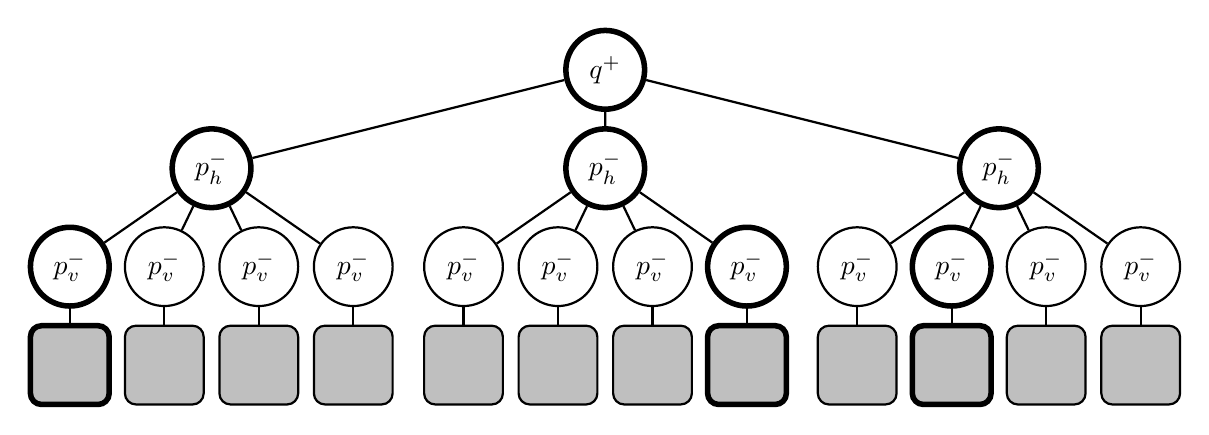
\begin{tikzpicture}[
	scale = 1, transform shape, thick,
	every node/.style = {draw, circle, minimum size = 10mm},
	grow = down,  % alignment of characters
	level 1/.style = {sibling distance=5cm},
	level 2/.style = {sibling distance=1.2cm}, 
	level 3/.style = {sibling distance=1.2cm}, 
	emph/.style={edge from parent/.style={red,very thick,draw}, line width = 2pt},
	norm/.style={edge from parent/.style={black,thin,draw}},
	leaf/.style={shape = rectangle, rounded corners, fill = gray!50},
	level distance = 1.25cm
	]
	
	\begin{scope}[xshift=0cm]
	\node[emph] {$q^+$} 
	child { node [emph] {$p_h^-$}
		child {   node [emph] {$p_v^-$}
			child { node [leaf,emph]  {}}
		}
		child {   node [norm] {$p_v^-$}
			child { node [leaf]  {}}
		}
		child {   node [] {$p_v^-$}
			child { node [leaf]  {}}
		}
		child {   node [] {$p_v^-$}
			child { node [leaf]  {}}
		}
	}
	child { node[emph] {$p_h^-$}
		child {   node [] {$p_v^-$}
			child { node [leaf]  {}}
		}
		child {   node [] {$p_v^-$}
			child { node [leaf]  {}}
		}
		child {   node [] {$p_v^-$}
			child { node [leaf]  {}}
		}
		child {   node [emph] {$p_v^-$}
			child { node [leaf,emph]  {}}
		}
	}
	child { node[emph] {$p_h^-$}
		child {   node [] {$p_v^-$}
			child { node [leaf]  {}}
		}
		child {   node [emph]{$p_v^-$}
			child { node [leaf,emph]  {}}
		}
		child {   node [] {$p_v^-$}
			child { node [leaf]  {}}
		}
		child {   node [] {$p_v^-$}
			child { node [leaf]  {}}
		}
	};
	\end{scope}
	\end{tikzpicture}
	\caption[Virtual constraint library structure]{Virtual constraint library structure. Each leaf contains $n_qn_k$ primitives in a sorted array. A possible (worst-case) search path is indicated in bold. Note that only  one initial condition $q^+\in\tilde{Q}$ is pictured. The library contains many repetitions of this structure.}
	\label{fig:lib}
\end{figure}

The library is built using a hierarchical (forest) structure with each of the impact configurations in $\tilde{Q}$ at the top. Consider this the initial configuration of the robot. Connected to each root node are $n_x$ nodes representing a particular step length $p_h(\theta^-)$. To each of these nodes are connected $n_y$ edges, encoding the grid of step heights $p_v(\theta^-)$. These edges are sorted in ascending order of height. At each of the nodes reachable from these edges, we have an encoded step length and height. This is important since there is only one height for a given length which is applicable based on the terrain.

Each of these nodes is associated with a sorted array containing $n_qn_k$ applicable trajectories $q^+ \to q^-$, specified by Bézier coefficients as discussed in Section \ref{sec:bezconstraints}. These paths are able to be sorted based upon the ordering method introduced in Section \ref{sec:orderings}. The library is therefore conducive to an efficient search from a particular initial configuration $q^+$ to a trajectory $q^+ \to q^-$ on the basis of first matching step heights to the terrain at given step lengths, then searching through only the applicable constraints for a desired velocity or kinetic energy. Note that since the primitives are ordered, this search is completed in $\mathcal{O}(n_x\log(n_yn_qn_k))$ time. This is clearly preferable to the $\mathcal{O}\left((n_xn_yn_q)^2n_k\right)$ time of a search through an unstructured array of all primitives in $P$. We may again motivate the need to keep $n_x$ small; the worst-case search time is logarithmic in $n_y$, $n_q$ and $n_k$ but linear in $n_x$.

\subsection{Data stored per virtual constraint}
As discussed in the Section \ref{sec:algreqs}, the selection algorithm's ability to efficiently and practically produce sequences of motion primitives places requirements on the virtual constraint library to include particular data per VC. This data is critical to the success and practicability of the virtual constraints method of path planning. The data associated with each constraint is presented in Table \ref{tab:datavc}

\begin{table}
	\centering
	\begin{tabular}{ c | c | c | c }
		Data                               & Description               & Type                      & Storage method \\ \hline
		$\Gamma(\theta^c), \Psi(\theta^c)$ & Partial sol at crit point & Floating-point            & Per VC         \\
		$\Gamma(\theta^-), \Psi(\theta^-)$ & Partial sol before impact & Floating-point            & Per VC         \\
		$\Gamma(\theta^+), \Psi(\theta^+)$ & Partial sol after impact  & Floating-point            & Per VC         \\
		$\Phi(\theta_0)$                   & Initial configuration     & Pointer into $\tilde{Q}$  & Per VC         \\
		$\Phi(\theta^-)$                   & Final configuration       & Pointer into $\tilde{Q}$  & Per VC         \\
		$s_l$                              & Step length               & Floating-point            & Tree structure \\
		$s_h$                              & Step height               & Floating-point            & Tree structure
	\end{tabular}
	\caption{Data associated with each virtual constraint in the library}
	\label{tab:datavc}
\end{table}

\subsection{Library generation algorithm}
The \mcode{generateLibrary} function is implemented in MATLAB to allow for simple interfacing with the simulation and optimisation code. However, the algorithm is more suited to languages with explicit pointers (e.g. C/C++), for reasons which should become apparent. The high-level structure of the algorithm is presented in Algorithm \ref{alg:highlevellib}.

\begin{algorithm}
\begin{algorithmic}[1]
	\Function{generateLibrary}{$n_x,n_y,n_q,n_k,deg,N_g,\dot{\theta}_a$}
		\State [$\tilde{Q}, \tilde{Q}_{tree}$] $\gets$ \Call {impactConfigs}{$n_x,n_y,n_q$}
		\State $\Delta$KE$_{list}$ $\gets$ \Call {DelKEs}{$n_k$}
		\State $P \gets$ emptyList
		\ForAll {$q^+ \in \tilde{Q}$}
			\State $L(q^+) \gets \tilde{Q}_{tree}$
			\ForAll {$len \in L(q^+).lens$}
				\ForAll {$ht \in L(q^+).len.hts$}
					\State $L(q^+).len.ht.prims \gets$ emptyArray($n_qn_k$)
					\ForAll {$q_n^+ \in L(q^+).len.ht.qs$}
						\State $q^- \gets Rq_n^+$
						\State $\sigma(x) \gets$ \Call {makeGround}{$q^+,q^-$}
						\ForAll {$\Delta$KE $\in$ $\Delta$KE$_{list}$}
							
							\State $[p, f] \gets$ \Call {optimiseVC}{$q^+,q^-,\Delta\mathrm{KE},\sigma(x),deg,N_g$}
							\If {$f \neq$ FAIL}
								\State $p.q^- \gets q^-$
								\State $p.q^+ \gets q^+$
								\State \Call{addToList}{$P, p$}
								\State \Call{addToArray}{$L(q^+).len.ht.prims, p$}
							\EndIf
						\EndFor
					\EndFor
					\State \Call {sortVCs}{$L(q^+).len.ht.prims, \dot{\theta}_a$}
				\EndFor
			\EndFor
		\EndFor
		\State \Return{$L,P,\tilde{Q}$}
	\EndFunction
\end{algorithmic}
\caption{Virtual constraint library generation}
\label{alg:highlevellib}
\end{algorithm}

The library generation begins by producing the set of impact configurations and a list of mutations in kinetic energy. Note that the impact configurations are returned both as an array and a tree; the tree is structured in the same manner as the virtual constraint library in order to enable its efficient generation. That is, the tree contains pointers to elements of $\tilde{Q}$, arranged by step length and then by height. For each element $q^+ \in \tilde{Q}$, the tree is duplicated and for each configuration $q^-$ at the leaf of the tree, $n_k$ virtual constraints are constructed which define paths $q^+ \to q^-$. These constraints are stored in a large structure $P$ containing all constraints. The leaves of the tree $L$, the library of virtual constraints, are arrays containing pointers to elements of $P$. This array is sorted using the ordering in Section \ref{sec:orderings}. %
\nomenclature{$\tilde{Q}$}{Set of all impact conditions in the virtual constraint library} %
\nomenclature{$P$}{The set of all primitives in the virtual constraint library} %
\nomenclature{$L$}{The structured virtual constraint library containing pointers into $\tilde{Q}$ and $P$}

\subsubsection{Impact configurations}
In order to generate the impact configurations in the form described above, it is necessary to calculate the inverse kinematics (IK) using a stipulated the step length and height. This significantly increases the complexity of the problem; forward kinematics (FK) are always able to be analytically derived, whereas one cannot even guarantee the existence of an IK solution. It is typically necessary to fix some other coordinates in order to produce a unique solution to the IK. %
\nomenclature[*]{IK}{Inverse kinematics; i.e. calculating a set of generalised coordinates $q$ to achieve a desired position of a point on the robot}

The IK are solved using a search with iterative grid refinement, as shown in Algorithm \ref{alg:iksol}. $s_l$ and $s_h$ are the step length and height respectively and $[h_h^*, h_v^*]$ is the position of the hip at impact. $N_g$ is the 1-D length of the grid, $\epsilon^*$ being the tolerance for error for accepting a solution. $q_p$ is the portion of the generalised coordinates which affect the position of the end of the swing leg $p$. 
\begin{algorithm}
\begin{algorithmic}[1]
	\Function {solveIK}{$s_l,s_h,h_h^*,h_v^*,N_g,\epsilon^*$}
		\State $[q_{p_{lim-}},q_{p_{lim+}}] \gets$ \Call{getLims}{}
		\State $q_p \gets (q_{p_{lim-}}+q_{p_{lim+}})/2$
		\State $q_{p_\Delta} \gets q_p - q_{p_{lim-}}$
		\State $i \gets 0$
		\State $accept \gets$ \textbf{false}
		\While {$\neg ~accept$}
			\State $q_{p_{min}} \gets q_p - q_{p_\Delta} / (\tfrac{1}{2}N_g)^i$
			\State $q_{p_{max}} \gets q_p + q_{p_\Delta} / (\tfrac{1}{2}N_g)^i$
			\State $[q_p,accept] \gets$ \Call{minGrid}{$s_l,s_h,h_l,q_{p_{min}},q_{p_{max}},N_g,\epsilon^*$}
			\State $i \gets i + 1$
		\EndWhile
		\State \Return{$q_p$}
	\EndFunction
	\Function {minGrid}{$s_l,s_h,h_h^*,h_v^*,q_{p_{min}},q_{p_{max}},N_g,\epsilon^*$}
		\State $[q_1, \ldots, q_n] \gets$ \Call{ndGrid}{$q_{p_{min}}^*,q_{p_{max}}^*,N_g$}
		\State $[p_h, p_y] \gets$ \Call{endSwingLeg}{$q_1, \ldots, q_n$}
		\State $[h_h, h_v] \gets$ \Call{hipPos}{$q_1, \ldots, q_n$}\Comment{Note hipPos ignored for CG}
		\State $\epsilon \gets \lVert [s_l-p_h; s_h-p_v; h_h^*-h_h; h_v^*-h_v] \rVert_2$
		\State $[\epsilon_{min}, q_{min}] \gets$ \Call{findMin}{$\epsilon$}
		\State \Return{$q_{min}, (\epsilon_{min} \leq \epsilon^*)$}
	\EndFunction
\end{algorithmic}
\caption{Iterative grid search for IK solution}
\label{alg:iksol}
\end{algorithm}

Setting the step length and height along with the hip position is sufficient to provide a unique solution to the IK for the legs of a planar bipedal robot with up to one knee per leg. Since coordinates above the hip, e.g. the torso angle, do not affect the step length and height, these may be freely chosen. Note that for each step length and height, $n_q$ different sets of hip height and applicable additional coordinates are set. For the degenerate case of the compass-gait walker, $n_q=1$, and the hip position is not constrained, since the step length and height are sufficient to uniquely define the IK.

It should be noted that this algorithm is exponential in the dimensions of $q_p$ and recalculates the entire grid each time. It is not possible in general to produce a polynomial time algorithm for IK \cite{??}, however the efficiency could be improved by using previous solutions to the IK to inform the initial guess, or by implementing an Adaptive Neuro-Fuzzy Inference System (ANFIS) \cite{??}.

It is important to check that the generated final configuration will be admissible on the basis of the simplified friction cone condition (Equation \ref{eqn:zeroslopefriccone}). This check may be completed in the code which calls \mcode{solveIK}. It is preferable that there are exactly $n_q$ configurations per step length and height in the library, so at this point the best practice is to recalculate the IK using a different set hip height or other coordinates. However, such configurations can be simply omitted from the library for simplicity of implementation without compromising the data structure. This is not a large concern; the friction cone constraint is typically satisfied if the range of step lengths and heights are within the robot's nominal operating limits.

The library of virtual constraints $L$ allows for an efficient search through the structure from a given initial configuration $q^+$. Since the virtual constraints contain references to the following impact configuration, finding the root in $L$ of a primitive given the preceding primitive is achieved in $\mathcal{O}(1)$ time. However, this clearly does not apply to the initial case. $\tilde{Q}$ is therefore sorted by $q_1$, then $q_2$, etc, to $q_n$. This allows for a $\mathcal{O}(\log\lvert\tilde{Q}\rvert)$ time initial search for a root node in $L$, assuming that the initial $q$ is known.

\subsubsection{Kinetic energy mutations}
The range of kinetic energy additions and subtractions must be set based upon the dynamics of the robot. This is intuitively obvious; a more massive robot with greater inertia requires a larger range of kinetic energy additions and subtractions. It therefore makes sense to define the kinetic energy mutations based upon the desired velocity characteristics, since these are much more intuitive and universal. The  maximum $\Delta$KE value is set by choosing the maximum change in generalised coordinate velocity $\delta\dot{q}_{max}$:
\begin{equation}
	\Delta\mathrm{KE}_{max} = (\delta\dot{q}_{max})^T M (\delta\dot{q}_{max})
\end{equation}
It is possible to formulate a less ``manual'' expression, in terms of the desired change in average horizontal velocity or similar, however since the change in kinetic energy is approximate and based only on a single constraint, it is deemed not necessary to commit computational power to solving such a formulation. The range in $\Delta$KE is produced by linear interpolation of $n_k$ values on the interval $[-\Delta\mathrm{KE}_{max},\Delta\mathrm{KE}_{max}]$.

\subsubsection{Ground definition}
Following the discussion in Section \ref{sec:ground} on conservative ground definitions, the ground height for all pairs of impact configurations $q^+, q^- \in \tilde{Q}$ is defined to be the following:
\begin{equation}
	\arraycolsep=1.4pt\def\arraystretch{1.5}
	\sigma(x) = \left\{
		\begin{array}{l c l}
			p_v(\theta^+) &~:~& x < \tfrac{1}{2}p_h(\theta^+) \\
			0 &~:~& x \in \left[\tfrac{1}{2}p_h(\theta^+), \tfrac{1}{2}p_h(\theta^-)\right) \\
			p_v(\theta^-) &~:~& x \geq \tfrac{1}{2}p_h(\theta^-)
		\end{array}
	\right.
\end{equation}
Optimising a virtual constraint with this ground definition implicitly enforces \ref{item:liftoff} and \ref{item:posnormalF} from Section \ref{sec:impact}, since if the configuration path leaves the ground on a positive-height trajectory, then comes back into contact with the ground from above, the vertical component of the swing foot's velocity, $p_v$, must be respectively positive and negative. The only robots which must have additional checks placed on the optimisation solution, therefore, are those with rigid legs, e.g. the compass-gait walker.

{\color{red}\subsubsection{Multiple orderings?}
Possibly order multiply in $\theta_c$ or perhaps also by $\theta^+$}

\subsubsection{MATLAB implementation}
Due to a lack of pointers in MATLAB, the set of all virtual constraints $P$ is stored in an array, with indexes operating as \textit{de facto} pointers. The same is true for the ``pointers'' in $\tilde{Q}_{tree}$ into $\tilde{Q}$. While this limits the freedom of memory allocation and precludes the program from several efficiency measures, the full functionality of the algorithm is able to be maintained.

The only significant point of difference in the algorithm is in the handling of the optimisation returning an invalid constraint or an error flag. Since the virtual constraint set $P$ must already be initialised and is indexed, it is necessary to fill the entries of $P$ corresponding to errors with some values. For reasons which should be self-evident when considering the ordering method in Section \ref{sec:orderings}, these entries are filled with $\Gamma_\bullet = 0, \Psi_\bullet=-\infty$.